\chapter*{Preface}

\begin{flushright}
``I remember when your project was just an 8051'' - Vimal Bhalodia
\end{flushright}

\vspace{0.8in}

Soma is a high-density recording system for real-time acquisition and
analysis of extracelluar electrophysiological signals. Here I describe
the design, implementation, and evaluation of the Soma Acquisition Board, 
an 8-channel low-latency amplifier for amplification and digitization
of these signals. The Acquisition Board feeds into the "Analysis" subsystem
consisting of the Soma DSP Modules, Backplane, and Network Interface,
which in turn transmit packetized filtered data out over the network. 

\begin{center}
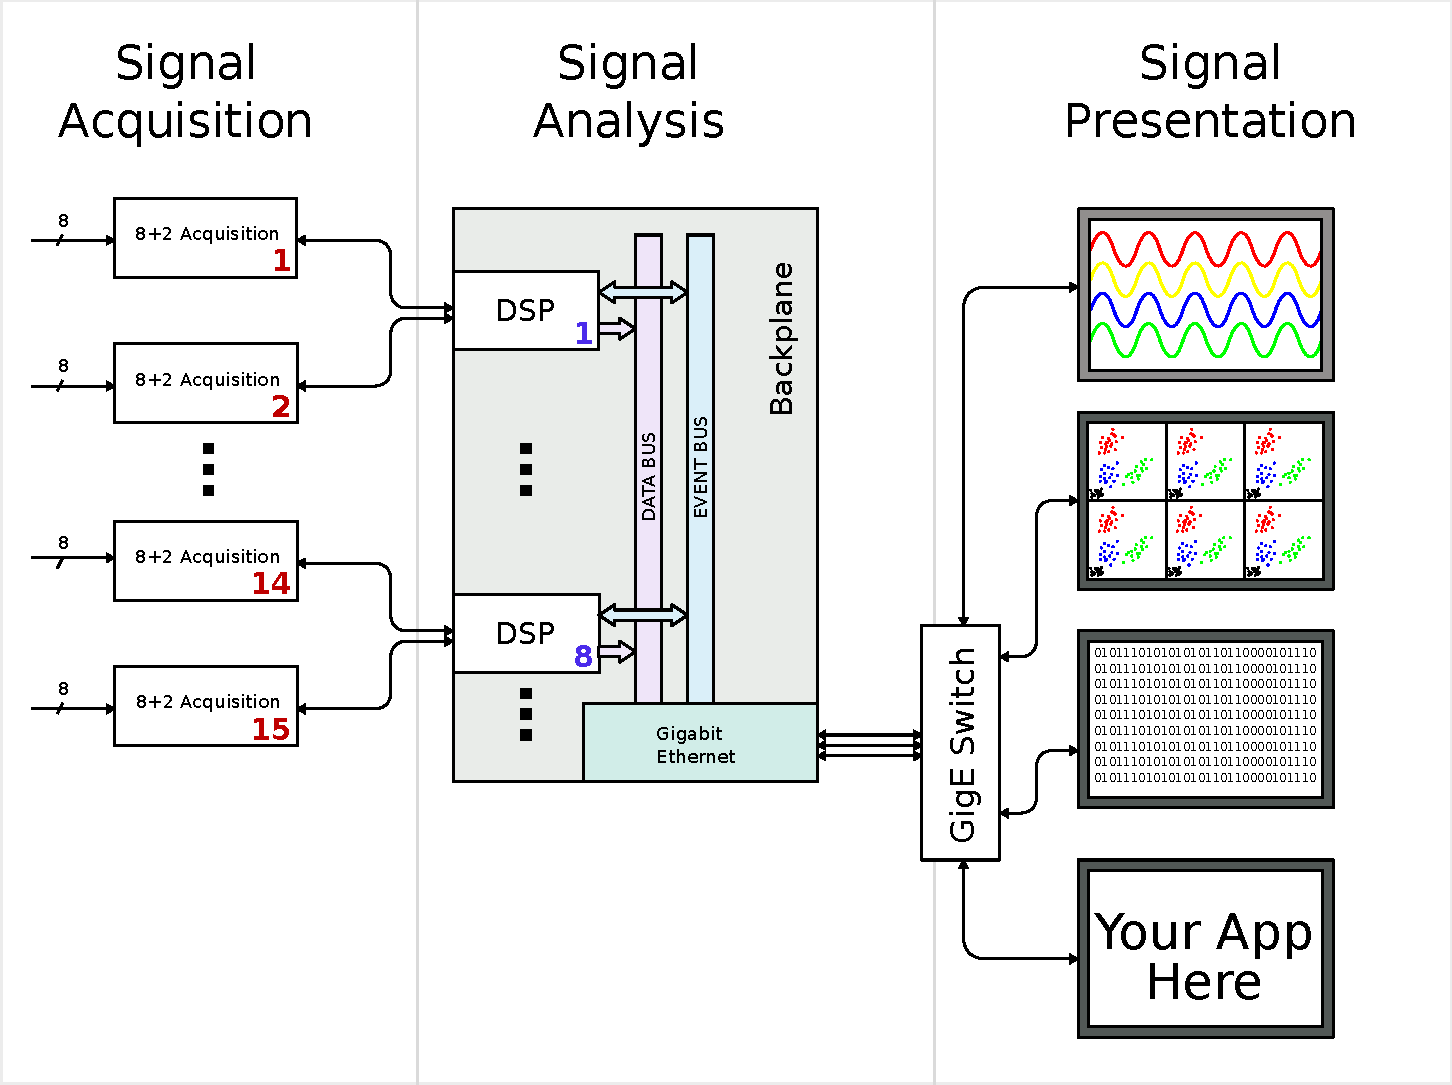
\includegraphics[width=4in]{arch.pdf}
\end{center}

The Acquisition Board was the first part of Soma that I designed, and
in many ways is the most complex. Mixed-signal design is always a
headache, and the acquisition board is no exception -- the
bill-of-materials lists over four hundred components, driven by six
different power supply rails.  Simply figuring out how to test the
board was a challenge, culminating in us purchasing a \$10,000 signal
generator traditionally used for measuring the performance of high-end
audiophile equipment.

I can't say there weren't mistakes along the way, or that knowing what
I know now, I wouldn't have done things differently. But the
acquisition board is versatile enough that, if I'm lucky, I may never
have to design another electrophysiology amplifier again. Thus, this
document, and the associated source code (available at
http://github.com/somaproject/acqboard ) should be viewed as a
reference design for others looking to implement similar designs.



\subsection*{Acknowledgments}

Soma began as an M. Eng. and grew into something much
larger. The extensive engineering involved would not have been
possible were it not for the support and encouragement of my parents
over all these years. They were willing to tolerate their seven-year-old's
solder fumes and incessant requests to buy parts at Radio Shank, and
encouraged me to embrace my curiosity and follow my passions (even
if they couldn't help me with the specifics of the NE555 timer IC). 

So thank you, Mom and Dad -- I know my MIT journey has taken longer
than any of us anticipated, but I hope you'll agree that it's been
worthwhile.

\vspace{0.5in}
Eric Jonas, 
August 20 2009
